\documentclass[10pt,a4paper]{article}

\usepackage{amsmath}
\usepackage{graphicx}
\usepackage{float}
\usepackage[polish]{babel}
\usepackage[utf8]{inputenc}
\usepackage{polski}
\usepackage{listings}
\frenchspacing
\lstset{basicstyle=\ttfamily,
  showstringspaces=false,
  breaklines=true,
  numbers=left,
  captionpos=b,
  language=bash,
  frame=single
}

\author{Marcin Ochman}
\title{Grafy - algorytmy wyszukiwania}

\begin{document}
\maketitle

\begin{figure}[H]
\centering
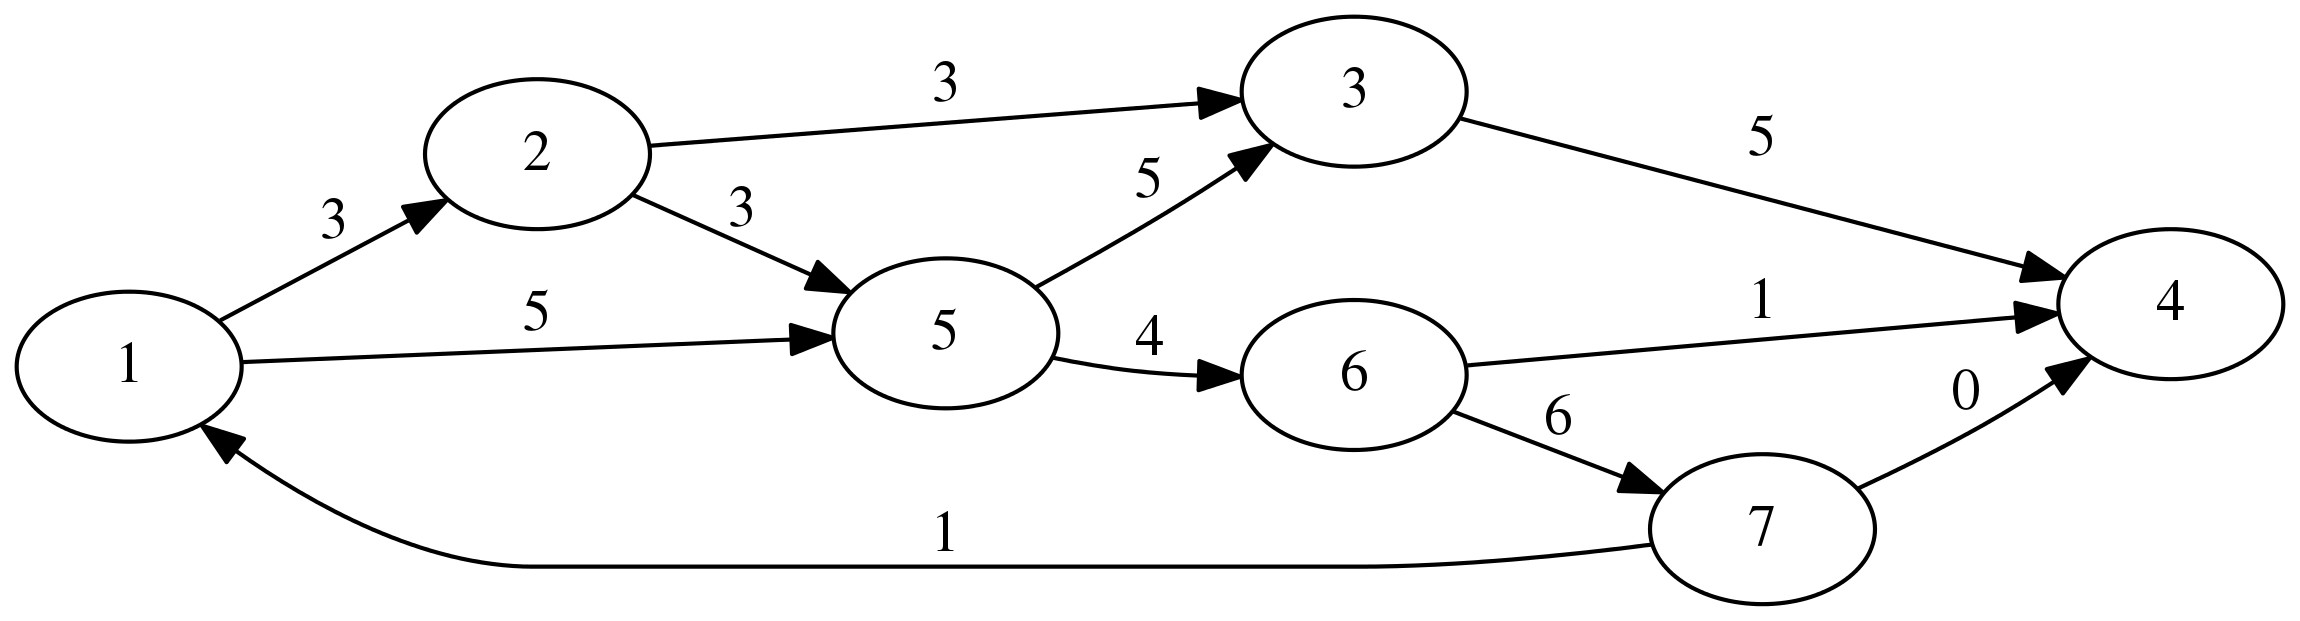
\includegraphics[width=0.7\linewidth]{./Wykresy/graf1}
\caption{Graf, który został użyty do testowania algorytmów przeszukiwania}
\label{fig:graf}
\end{figure}

\begin{figure}[H]
\centering
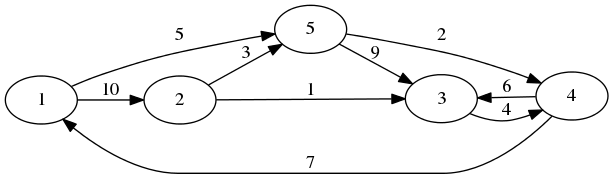
\includegraphics[width=0.7\linewidth]{./Wykresy/graf2}
\caption{Drugi graf, który został użyty do testowania algorytmów przeszukiwania}
\label{fig:graf}
\end{figure}

\section{Opis problemu}
Jednym z najczęstszych problemów, z którymi można się spotkać w
świecie grafów to problem wyszukiwania ścieżki z wierzchołka 
startowego do wierzchołka końcowego. Dodatkowo,
najczęściej interesuje nas najkrótsza ścieżka, ale czasami 
wystarczy, że algorytm znajdzie tylko taką ścieżkę, która zaprowadzi
nas z określonego miejsca do punktu docelowego. Na laboratorium
zaimplementowałem cztery różne algorytmy przeszukiwania, przy czym
ostatni znajduje optymalną ścieżkę tzn. koszt jest najmniejszy.
Są to:
\begin{itemize}
\item DFS - deep first search
\item BFS - breadth first search
\item Best First Search
\item A*
\end{itemize}

\section{Opis poszczególnych algorytmów}


\begin{figure}[H]
\centering
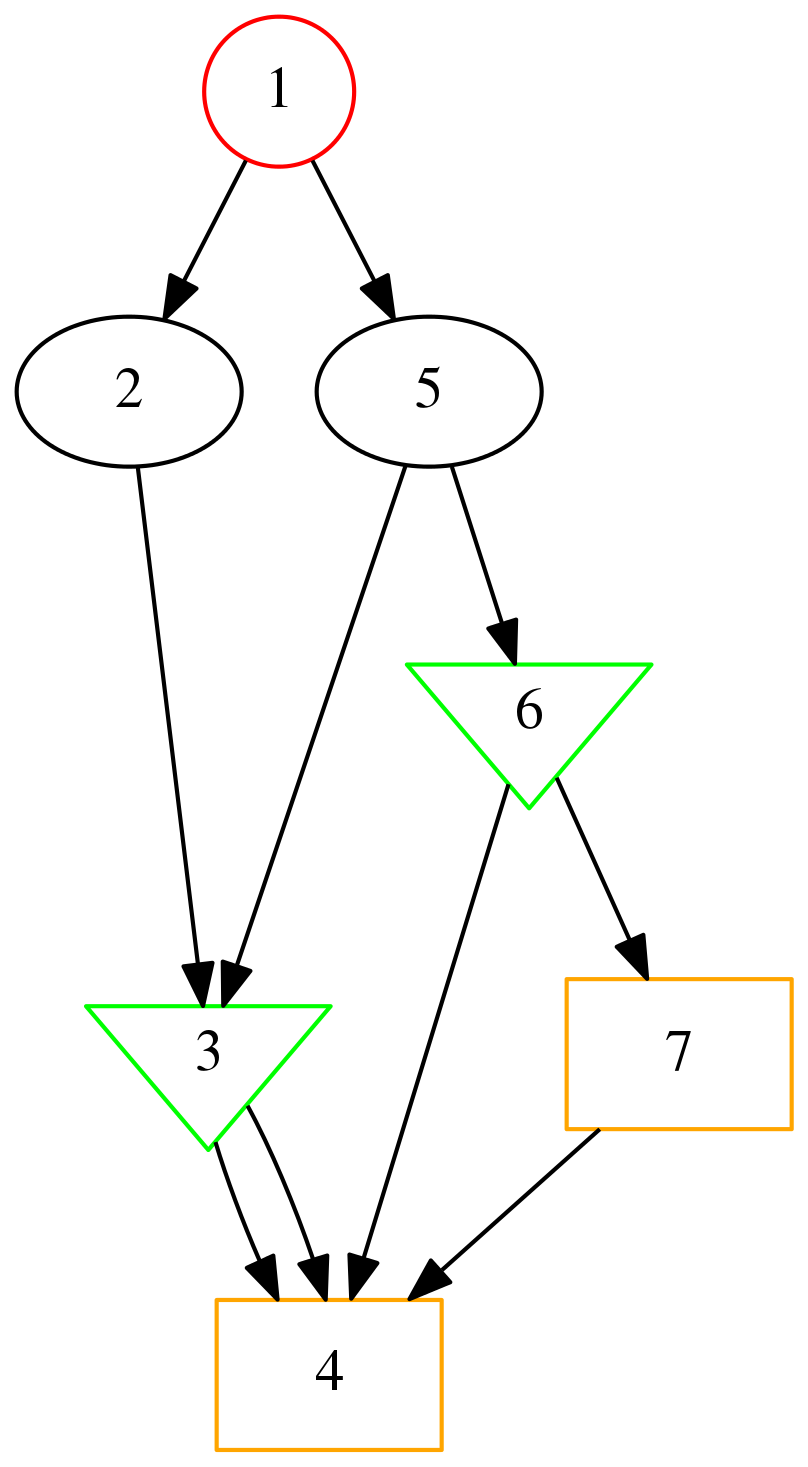
\includegraphics[height=0.7\linewidth]{./Wykresy/drzewo}
\caption{Drzewo, które zostało zbudowane w oparciu o graf z 
Rysunku \ref{fig:drzewo}. Każdy poziom został wyróżniony różnym 
kształtem oraz kolorem }
\label{fig:drzewo}
\end{figure}


Każdy z algorytmów działa nieco inaczej. Postaram się w kilku
słowach opisać, jak funkcjonuje każdy z nich.

\subsection{DFS - Deep First Search}
Jak sama nazwa wskazuje algorytm przeszukuje graf w
głąb tzn. najpierw brane są pod uwagę wierzchołki, które są
sąsiadami danego wierzchołka - procedura wykonuje się rekurencyjnie.
Na drzewie na Rysunku \ref{fig:drzewo} przeszukiwań można powiedzieć, że algorytm przechodzi
najpierw w dół, następnie wraca do wierzchołka i powtarza procedurę.
Każdy poziom jest odwiedzany kilkakrotnie.

\subsection{BFS -Breadth First Search }
Polska nazwa tego algorytmu to wyszukiwanie wszerz. Polega on na
odwiedzaniu wierzchołkow należących do tego samego poziomu, a
następnie schodzi on poziom niżej.


\subsection{Best First Search}
Jest to algorytm zachłanny - odwiedza pierwszy ten wierzchołek, 
który spełnia pewne kryterium np. minimalne waga połączenia z 
poprzednim wierzchołkiem.

\subsection{A*}
Jest to algorytm oparty na funkcji heurstycznej. Na jej podstawie
potrafi dobierać, która ścieżka jest najlepsza w odpowiednim momencie. Dla określonych funkcji heurstycznych mamy gwarancję, że
zozstanie znaleziona optymalna ścieżka. Algorytm ten jest często 
używany w grach. Dla funkcji heurystycznej, która zawsze zwraca 0,
algorytm ten sprowadza sie do algorytmu Dijkstry.

\section{Porównanie poszczególnych algorytmów w praktyce}

Do porównania działania algorytmów posłużyłem się grafem z Rysunku \ref{fig:graf}.
Zadaniem było znalezienie ścieżki z wierzchołka 1 do 4.
Poszczególne ścieżki, dla różnych algorytmów zostały przedstawione
na Listingu

\begin{lstlisting}[caption={Wyniki poszukiwania ścieżek dla poszczególnych algorytmów}]
Graf nr 1:

A*:
1->5->6->4
DFS:
1->5->6->7->4
BFS:
1->2->3->4
Best First Search:
1->2->3->4

Graf 2:

A*:
1->5->4->3
DFS:
1->5->4->3
BFS:
1->2->3
Best First Search:
1->5->4->3
\end{lstlisting}

\section{Wnioski oraz uwagi}

Na podstawie przeprowadzonych testów można wysnuć następujące wnioski:
\begin{itemize}
\item Algorytm A* faktycznie znalazł najkrótszą ścieżkę, funkcja
heurystyczna zawsze zwracała 0
\item Algorytm Best First Search za każdym razem wybierał
drogę, która była najmniej kosztowna
\item Budowa grafu ma duży wpływ na to, który algorytm DFS, BFS oraz Best First Search będzie lepszy tzn. pokaże lepsza ścieżkę
\end{itemize}

\end{document}